\chapter{Arhitektura i dizajn sustava}
		
	
	Arhitektura ovog projekta se može razlučiti na tri podsustava:
	\begin{packed_item}
	\setlength\itemindent{24pt}
		\item\textbf{Web aplikacija}
		\item\textbf{Web poslužitelj}
		\item\textbf{Baza podataka}
	\end{packed_item}
	
	\textbf{Web poslužitelj} je podsustav kojemu je zadaća spremanje, obrađivanje i dostavljanje klijentima sadržaj web stranica. Preko web aplikacije poslužitelj komunicira sa klijentom koji je u ovom slučaju web preglednik. Komunikacija se odvija putem protokola aplikacijskog sloja interneta - HTTP (Hypertext Transfer Protocol). On je tu da "reagira" na akcije koje mu web preglednik proslijedi te o ovisno o potrebi proljeđuje zahtjev na web aplikaciju.\\
	
	\textbf{Web preglednik} je program koji fizičkom korisniku omogućuje učitavanje i pregled web aplikacije. On je tu kao prevoditelj što znači da interpretira prikaz koda pisanog i uređivanog u HTML-u u izgled razumljiv
korisnicima. Putem web preglednika korisnik šalje HTTP zahtjeve web poslužitelju, no isto tako web poslužitelj je tu da prilagodi prikaz HTTP odgovora i prikaže ih korisniku.\\

	\textbf{Baza podataka} je podsustav u podatkovnom sloju kojem je primaran uloga sigurno spremanje podataka, a detaljnije o njoj se govori u poglavlju 4.1.\\
	
	\textbf{Web aplikacija} je dio sustava kojeg korisnik koristi za obrađivanje željenih zahtijeva koji uzrokuju pristupanje podacima u bazi podataka. Web aplikacija za interpretiranje dostavlja web pregledniku određeni HTML kod, a podijeljena je na back-end i na front-end o kojima je riječ u nastavku.
	\begin{packed_item}
	\item\textbf{Front-end} ili klijentska strana je dio aplikacije koji služi za sve ono vidljivo na web pregledniku. On je prezentacijski sloj koji korisniku omogućuje jednostavnu komunikaciju sa sustavom. Tehnologija koja je korištena za realizaciju ovog dijela web aplikacije je programski jezik JavaScript, preciznije radni okvir React u kombinaciji sa TypeScriptom.
	\item\textbf{Back-end} ili poslužiteljska stran je dio aplikacije koji je zadužan za obrađivanje dobivenih zahtjeva i vršenja funkcionalnih akcija. Tehnologija u kojom je pisan je programski jezik Java, preciznije u radnom okviru SpringBoot.\\
	\end{packed_item}

	Okruženje u kojem je pisan front-end je Visual Studio Code, a backe-end u Intellij-u. To nisu fiksna okruženja i može se koristiti bilo koji drugi IDE ili text editor. Arhitektura sustava se temelji na višeslojnom arhitekturnom stilu koji je podržan od strane SpringBoot tehnologije.\\
	
	\textbf{\underline{Višeslojni stil arhitekture}}\\
	Višeslojna arhitektura sastoji se od idućih slojeva:
	\begin{packed_item}
	\setlength\itemindent{24pt}
	\item klijentske strane koja omogućuje prikaz korisničkog sučelja
	\item nadglednika koji korisničku i poslužiteljsku stranu
	\item usluge koja obavlja poslovnu logiku i ostvaruje temeljnu funkcionalnost i zadaaću web aplikacije
	 \item repozitorija koji definira način pristupanja podacima
	 \item baze podataka koja u našem slučaju podatke sprema u relacijsku bazu Postgre\\
	\end{packed_item}
	
	Osnovna značajka ovakvog stila arhitekture su da svaki sloj pruža uslugu drugom sloju, a skriva svoj skup usluga. Jedna od prednosti ovog stila je olakšavanje ostvarivanja podjele brige u web aplikaciji jer se svaki sloj brine isključivo o svojoj funkcionalnosti. Klijentska strana razgovara sa web sučeljem, nadglednik putem REST API-ja pruža vanjsko sučelje i prihvaća HTTP zahtjeve te poziva odgovarajuće usluge, a potom te iste vraća kao odgovor klijentu. Sloj usluge definira pristup uslugama web aplikacije(tko i kako pristupa). Sloj repozitorija nam osigurava pristup podacima, te preslikavanje domenskih objekata u bazu podataka koristeći formu 1:1. Skica ovakve arhitekure je dana na slici \ref{fig:arhitektura}\\
	
	\begin{figure}[H]
			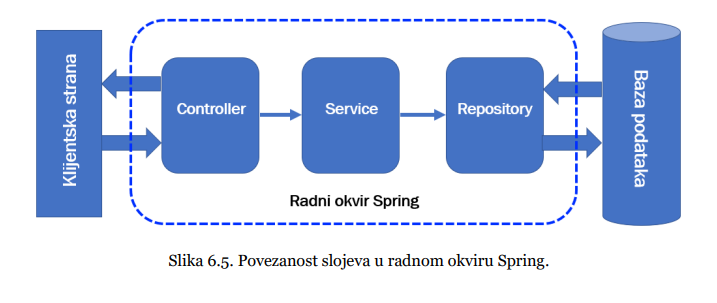
\includegraphics[scale=0.8]{slike/viseslojna_arhitekt.PNG} %veličina slike u odnosu na originalnu datoteku i pozicija slike
			\centering
			\caption{Primjer višeslojne arhitekture korištenjem radnog okvira Spring}
			\label{fig:arhitektura}
		\end{figure}

	
		

		

				
		\section{Baza podataka}
			
			\textbf{\textit{dio 1. revizije}}\\
			
		Za potrebe sustava koristit će se relacijska baza podataka koja nam omogućuje jednostavnije modeliranje stvarnog svijeta. Baza je implementirana u PostgreSQL-u zbog njegove jednostavnosti i jer je tim najbolje upoznat s tim sustavom; njegovim limitacijama i pravilima. Entiteti stvarnog svijeta su prevedeni kao tablice (relacije) koje imaju ime i svoj skup atributa. Baza podataka osigurava nam jednostavnu pohranu, umetanje, izmjenu i dohvat podataka, te garantira njihovu sigurnost. Baza podataka koristi sljedeće atribute:
		\begin{packed_item}
		\setlength\itemindent{24pt}
		\item prijave
		\item lokacije
		\item slike
		\item sorisnici
		\item tipovi{\_}ostecenja
		\item gradski{\_}uredi
		\end{packed_item}
		
		
			\subsection{Opis tablica}
			

				\textbf{prijave} je entitet koji sadrži sve važne informacije o podnesenim prijavama. Sastoji se od atributa:id, ostecenje{\_}id, lokacija{\_}id, kreator{\_}id, parent{\_}prijava{\_}id, prvo{\_}vrijeme{\_}prijave,
vrijeme{\_}otklona, naziv, opis. Ovaj entitet u vezi je One-to-One s tablicom lokacije preko atributa lokacija{\_}id, sa entitetom slike je u vezi One-to-Many preko atributa id. Sa entitetom tipovi{\_}ostecenja je u vezi One-to-Many preko atributa ostecenje{\_}id, u vezi Many-to-One sa entitetom korisnici preko atributa kreator{\_}id, te je sama sa sobom u refleksivnoj vezi One-to-Many preko atributa id.\\
				
				
				\begin{longtblr}[
					label=none,
					entry=none
					]{
						width = \textwidth,
						colspec={|X[6,l]|X[6, l]|X[20, l]|}, 
						rowhead = 1,
					} %definicija širine tablice, širine stupaca, poravnanje i broja redaka naslova tablice
					\hline \SetCell[c=3]{c}{\textbf{prijave}}	 \\ \hline[3pt]
					\SetCell{LightGreen}id & INT & jedinstveni identifikator prijave  	\\ \hline
					\SetCell{LightBlue}ostecenje{\_}id	& INT & jedinstveni identifikator tipa ostecenja   	\\ \hline 
					\SetCell{LightBlue}kreator{\_}id & INT &  jedinstvani identifikator korisnika koji je poslao prijavu \\ \hline 
					\SetCell{LightBlue}parent{\_} prijava{\_}id & INT & jedinstveni identifikator prijave na koju se prijava nadovezala		\\ \hline 
					 prvo{\_}vrijeme\_ prijave	& INT &  vrijeme slanja prijave 	\\ \hline
					 vrijeme{\_}otklona	& INT &  vrijeme otklona prijave 	\\ \hline 
					 opis & VARCHAR &  opis poslane prijave 	\\ \hline
					 naziv	& INT &  konkretno ime poslane prijave 	\\ \hline
					\end{longtblr}
					
					\textbf{lokacije} je entitet koji sadrži osnovne podatke o geografskoj lokaciji pojedine prijave. Sastoji se od atributa: lokacija{\_}id, latitude, longitude. Preko atributa id je povezana vezom One-to-One sa relacijom Prijave.\\
				
				\begin{longtblr}[
					label=none,
					entry=none
					]{
						width = \textwidth,
						colspec={|X[6,l]|X[6, l]|X[20, l]|}, 
						rowhead = 1,
					} %definicija širine tablice, širine stupaca, poravnanje i broja redaka naslova tablice
					\hline \SetCell[c=3]{c}{\textbf{Lokacije}}	 \\ \hline[3pt]
					\SetCell{LightGreen}lokacija{\_}id & INT &  	jedinstveni identifikator prijave 	\\ \hline
					latitude & INT & geografska latituda lokacije   	\\ \hline 
					longitude & INT & geografska longituda lokacije   	\\ \hline 
				\end{longtblr}
				
				\textbf{korisnici} je entitet koji sadrži osobne podatke o registriranim korisnicima kao i njihovu pripadnost vijecu i ulogu koju obnašaju u sustavu. Sastoji se od atributa: id, ime, prezime, username, email, password, ured{\_}id, role, active. Povezani su sa relacijom prijave u vezi One-to-Many preko atributa id, te sa relacijom gradski{\_}uredi u vezi Many-to-One preko atributa ured{\_}id.\\
				
				\begin{longtblr}[
					label=none,
					entry=none
					]{
						width = \textwidth,
						colspec={|X[6,l]|X[6, l]|X[20, l]|}, 
						rowhead = 1,
					} %definicija širine tablice, širine stupaca, poravnanje i broja redaka naslova tablice
					\hline \SetCell[c=3]{c}{\textbf{korisnici}}	 \\ \hline[3pt]
					\SetCell{LightGreen}id & INT & jedinstveni identifikator korisnika  	\\ \hline
					ime	& VARCHAR & ime registriranog korisnika   	\\ \hline
					prezime	& VARCHAR & prezime registriranog korisnika   	\\ \hline
					username	& VARCHAR & korisničko ime registriranog korisnika   	\\ \hline 
					email & VARCHAR & e-mail adresa registriranog korisnika   	\\ \hline
					password  & VARCHAR & lozinka za prijavu registriranog korisnika   	\\ \hline
					\SetCell{LightBlue}ured{\_}id & INT &  jedinstvani identifikator vijeca/ureda kojem pripada \\ \hline 
					active & INT & jedinstveni token sesije prijave korisnika		\\ \hline 
					 role & VARCHAR &  uloga koju korisnik obnaša u sustavu 	\\ \hline 
				\end{longtblr}
				
				\textbf{slike} je entitet koji sadrži podatke vezane za sliku podnešene prijave. Sastoji se od atributa: id, podatak, prijava{\_}id. Preko entiteta prijava{\_}id je povezan tablicom prijave u vezi Many-to-One.\\
				
				\begin{longtblr}[
					label=none,
					entry=none
					]{
						width = \textwidth,
						colspec={|X[6,l]|X[6, l]|X[20, l]|}, 
						rowhead = 1,
					} %definicija širine tablice, širine stupaca, poravnanje i broja redaka naslova tablice
					\hline \SetCell[c=3]{c}{\textbf{slike}}	 \\ \hline[3pt]
					\SetCell{LightGreen}id & INT &  	jedinstveni identifikator slike pojedine prijave	\\ \hline
					podatak & VARCHAR & string bitova koji sadrže sliku   	\\ \hline 
					\SetCell{LightBlue}prijava{\_}id & INT & jedinstveni identifikator prijave za koju je poslana slika   	\\ \hline 
				\end{longtblr}
				
				\textbf{tipovi{\_}osetecenja} je entitet koji sadrži podatke vezane za opis oštećenja kao i id ureda koji se bavi tim tipom oštećenja. Sastoji se od atributa: id, naziv. Preko atributa id je povezan sa relacijom prijave u vezi Many-to-One, te je sa relacijom gradski{\_}uredi u vezi One-to-One povezan preko istog atributa id.\\
				
				\begin{longtblr}[
					label=none,
					entry=none
					]{
						width = \textwidth,
						colspec={|X[6,l]|X[6, l]|X[20, l]|}, 
						rowhead = 1,
					} %definicija širine tablice, širine stupaca, poravnanje i broja redaka naslova tablice
					\hline \SetCell[c=3]{c}{\textbf{tipovi\_ ostecenja}}	 \\ \hline[3pt]
					\SetCell{LightGreen}id & INT &  	jedinstveni identifikator vrste oštećenja	\\ \hline
					naziv & VARCHAR & naziv konkretnog oštećenja   	\\ \hline  
				\end{longtblr}
				
				\textbf{gradski{\_}uredi} je entitet koji sadrži podatke vezane za opis pojedinog vijeca/ureda koji je zadužen za otklanjanje određenog tipa oštećenja. Sastoji se od atributa: id, naziv i ostecenje{\_}id. Preko atributa ostecenje{\_}id je povezan sa relacijom tipovi{\_}ostecenja u vezi Many-to-One, te je povezan sa relacijom korisnici preko atributa id u vezi One-to-Many.\\
				
				\begin{longtblr}[
					label=none,
					entry=none
					]{
						width = \textwidth,
						colspec={|X[6,l]|X[6, l]|X[20, l]|}, 
						rowhead = 1,
					} %definicija širine tablice, širine stupaca, poravnanje i broja redaka naslova tablice
					\hline \SetCell[c=3]{c}{\textbf{gradski{\_}uredi}}	 \\ \hline[3pt]
					\SetCell{LightGreen}id & INT &  jedinstveni identifikator pojedinog registriranog vijeća/ureda	\\ \hline
					naziv & VARCHAR & puni naziv vijćea u aplikaciji\\ \hline 
					\SetCell{LightBlue}ostecenje{\_}id & INT & identifikator vrste oštećenja koje za koje je taj ured zadužen\\ \hline
				\end{longtblr}
				
				
			
			\subsection{Dijagram baze podataka}
				\begin{figure}[H]
			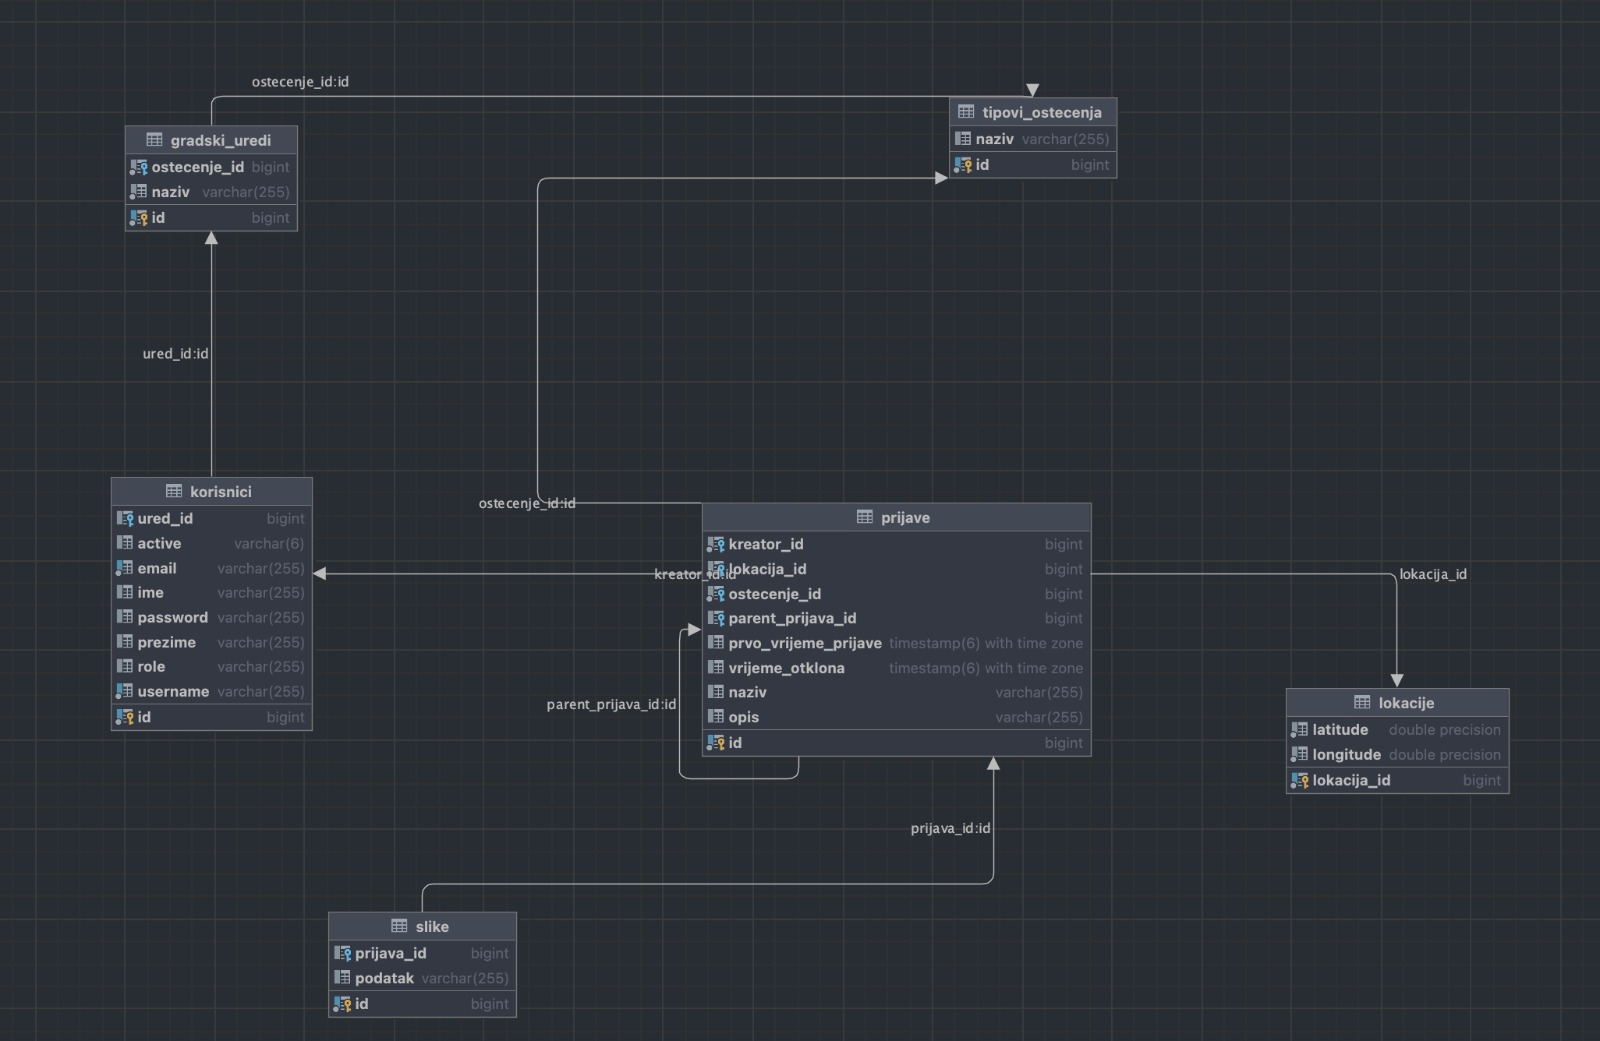
\includegraphics[scale=0.3]{slike/erBaza.PNG} %veličina slike u odnosu na originalnu datoteku i pozicija slike
			\centering
			\caption{Relacijski dijagram baze podataka}
			\label{fig:bazapod}
		\end{figure}
			
			\eject
			
			
		\section{Dijagram razreda}
		
			Na slikama 4.3 i 4.4 prikazani su razredi i njihove relacije na serverskoj strani aplikacije. Konkretnije rečeno prikazani su modeli i kontroleri. \\
			
			Svi kontroleri nasljeđuju razred Controller. Metode koje su u njima implementirane ovise o DTO objektima, koji se realiziraju pomoću metoda implementiranih u Domain dijelu razreda.
			
			
				\begin{figure}[H]
			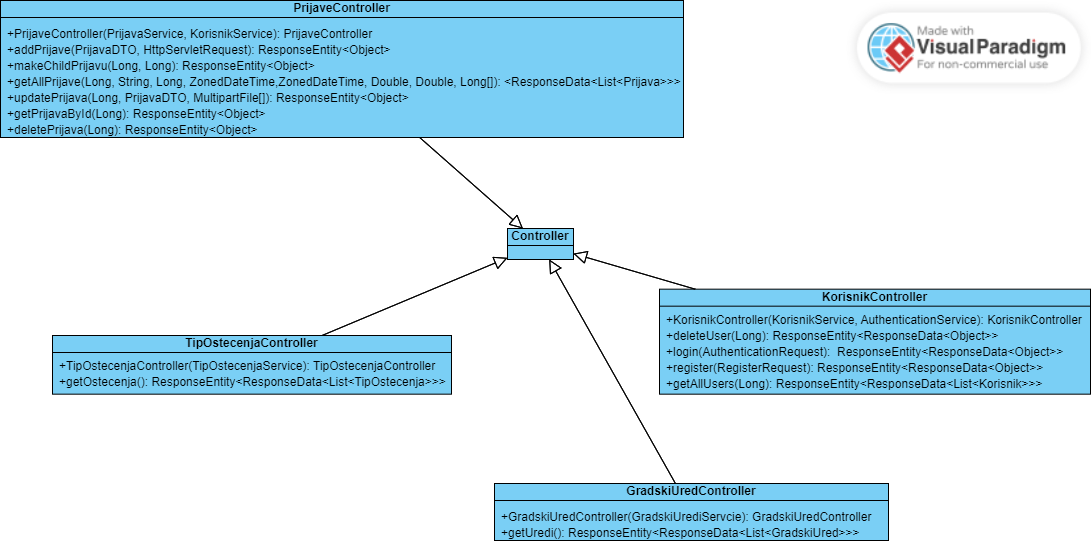
\includegraphics[scale=0.3]{slike/kontroleri.PNG} %veličina slike u odnosu na originalnu datoteku i pozicija slike
			\centering
			\caption{Dijagram razreda - Controllers dio}
			\label{fig:bazapod}
		\end{figure}
		
		\pagebreak
		
		Domain dio razreda preslikava strukturu baze podataka, te svi razredi nasljeđuju razred Model. Ovako ilustrirani razredi su zapravo odraz onih relacija koji su zapisani u bazi podataka, te direktno komunciraju sa bazom podataka. Razred Korisnik je ilustracija bilo kojeg registriranog usera koji ima svoju ulogu (povezan sa enumom Role), te može podnijeti prijavu u sustav (pvezanost sa razredom Prijava preko private atributa prijave). Prijave kada se konstruiraju zadaje im se lokacija (pa su preko atributa lokacija povezane sa razredom Lokacija), slika (agregatna povezanost sa razredom Slika preko varijable slike) i tip ostecenja (agregatna povezanost sa razredom tipOstecenja preko atributa tipOstecenja). Razred GradskiUred je reprezentacija gradskig ureda koje je povezan sa tipom oštećenja preko atributa tipOstecenja. \\
		
		
			\begin{figure}[H]
			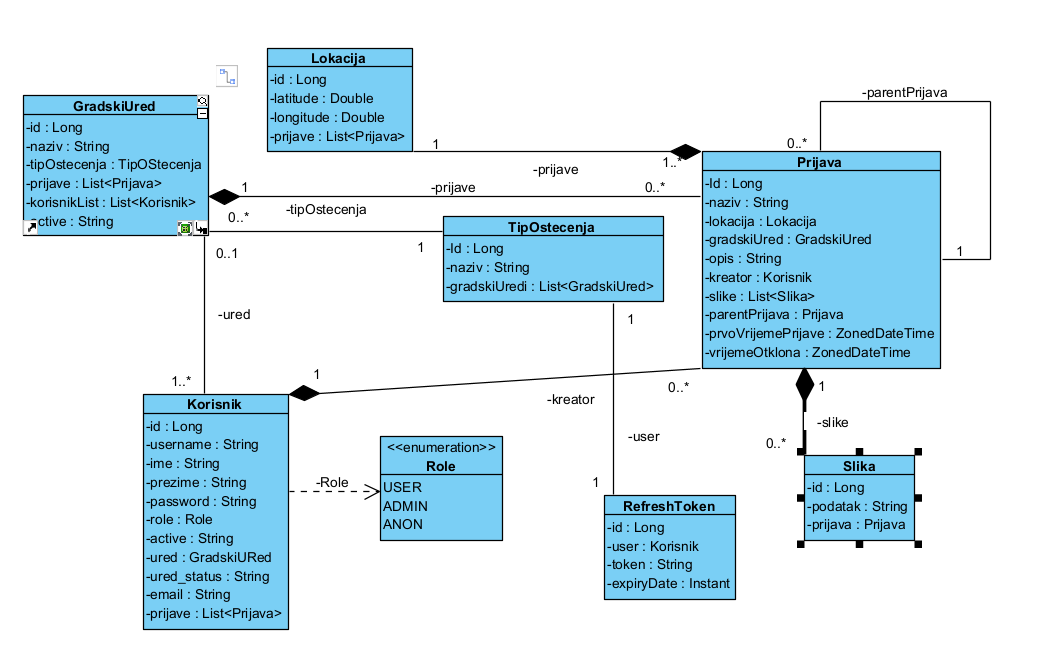
\includegraphics[scale=0.3]{slike/domain.PNG} %veličina slike u odnosu na originalnu datoteku i pozicija slike
			\centering
			\caption{Dijagram razreda - Controllers dio}
			\label{fig:bazapod}
		\end{figure}
			
			
			\eject
		\section{Dijagram stanja}
			
			
			Dijagrami stanja su tu da predoče stanja objekta, te prijelaze iz jednog stanja u drugo na poticaj nekakvog događaja (okidača). Na slici je prikazan dijagram stanja za prijavljenog korisnika. Korisniku je prikazana početna stranica sa Google Maps kartom na kojoj su ozačene prijave koje su aktivne, ali i opcija za podnošenje nove prijave kao i pretraga prijava po određenim filterima. Pri odabiru opcije za podnošenje nove prijave otvara mu se forma koja zahtijeva unos određenih podataka karakterističnih za vrstu  štete. Također, ako korisnik ne želi podnijeti novu prijavu u sustav, već po pretragama postojećih, može samo tu istu odabrati i klikom na "Pošalji" se ta ista prijava šalje opet u sustav. Nadalje, korisnik klikom na "Gradski uredi" može vidjeti listu postojećih gradskih ureda, ali i kreirati novi gdje mu se otavara forma koja zahtjeva unos podataka za novi ured. Korisnik u svakom trenutku može kliknuti na ikonicu profila i odabirom "Izmijeni profil" uređivati svoje podatke, ali i pregledati vlastite prijave klikom na "Pregled mojih prijava". Korisnik se iz sustava odjavljuje odabirom opcije "Odjava."
			
			
			\begin{figure}[H]
			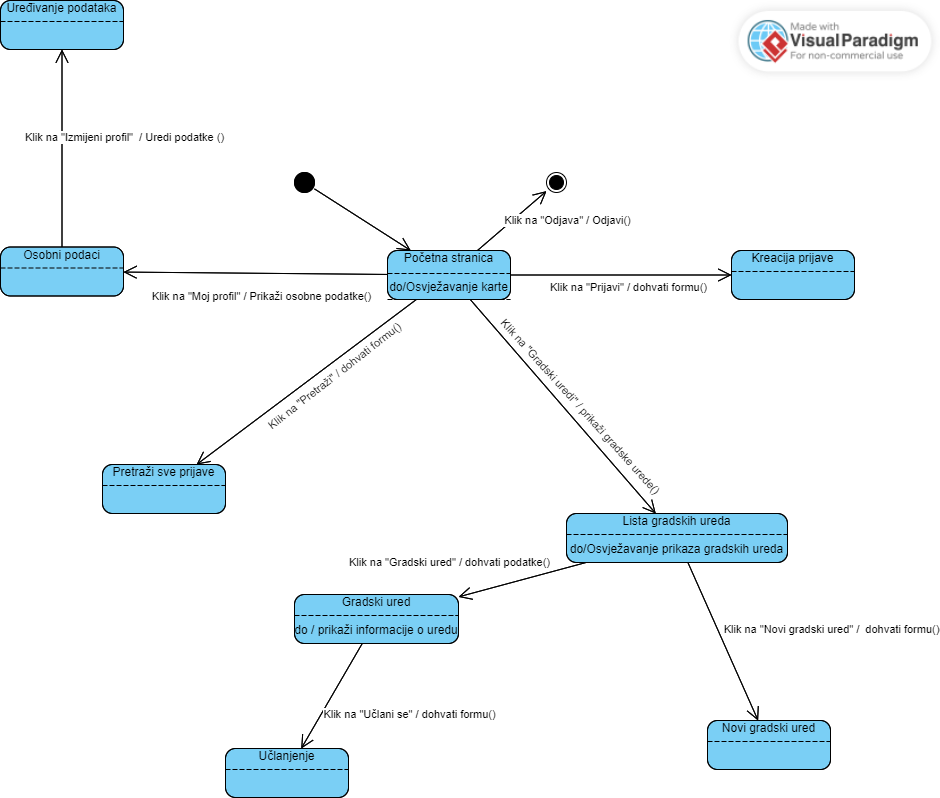
\includegraphics[scale=0.4]{slike/DijagramStanja.PNG} %veličina slike u odnosu na originalnu datoteku i pozicija slike
			\centering
			\caption{Dijagram stanja - Prijavljeni korisnik}
			\label{fig:bazapod}
		\end{figure}
			
			\eject 
		
		\section{Dijagram aktivnosti}
			
			Dijagram aktivnosti se koristi za opis modela toka upravljanja ili toka podataka. U modeliranju jednog takvog dijagrama aktivnosti, podrazumijeva se da se novi korak inicira tek kada prethodni završi. Na dijagramu prikazanom na idućoj slici prikazano je podnošenje prijave u sustav nakon logina korisnika. Korisniku se nakon opcije prijavi otvara forma sa traženim podacima. Kada unese tražene podatke, korisnik podnosi prijavu u sustav.
			
			
			\begin{figure}[H]
			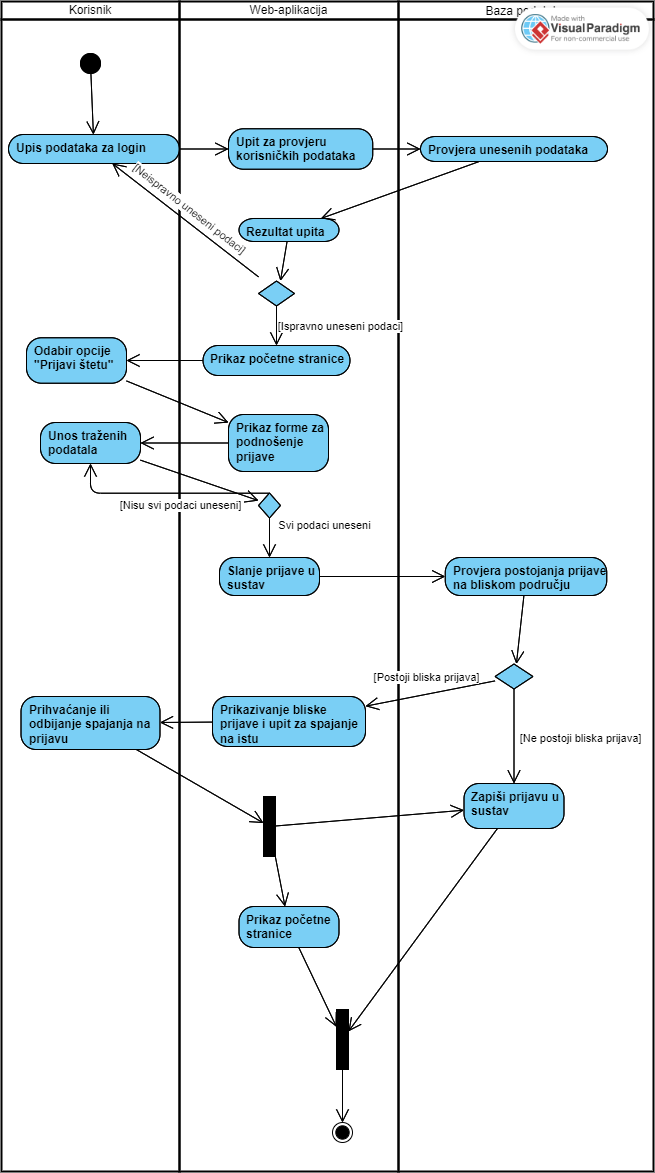
\includegraphics[scale=0.4]{slike/ActivityDiagram.PNG} %veličina slike u odnosu na originalnu datoteku i pozicija slike
			\centering
			\caption{Dijagram aktivnosti - Dodavanje prijave}
			\label{fig:bazapod}
		\end{figure}
			
			\eject
		\section{Dijagram komponenti}
		
			Dijagram komponenti nam pomaže slikovno ilustrirati ovisnost i razmještaj svih komponenti u sustavu. Dijagram predočen slikom 4.8. sastoji se od 3 glavne komponente: web preglednika kojim korisnik pristupa aplikaciji, frontend dijela zaduženog za interakciju sa kroisnikom i prosljeđivanje podataka backendu, te backend dijela koji vrši svu pozadinsku funkcionalnost aplikacije. Preko web sučelja se u web pregledniku prikazuju određeni "pogledi", tj. Router određuje koja će se stranica prikazati na osnovi upisanog URL-a. Ključne stvari od kojih se još frontend sastoji su index.ts, App.tsx i React JavaScript.  Sve TypeScript datoteke ovise o biblioteci React JavaScript koja dohvaća gotove komponente koje se koriste u interakcijama. index.ts je početni prikaz koji kominicira sa App.tsx-om koji dalje izgrađuje grafičko sučelje (poziva svoje specijalizacije) ovisno o korisnikovim akcijama. Kako bi se dohvatile JSON datoteke view komponenta preko REST API-ja komunicira sa backend dijelom sustava. Controller komponenta na backend strani prima podatke, ali i šalje odgovarajuće response poruke. Service komponenta prima zahtjeve od Controllera, obrađuje ih i prosljeđuje Repository komponenti koja preko JPA sučelja "izvlači" određene tablice iz baze podataka i pretvara ih u DTO oblik koje šalje opet u protok kroz arhitekturu.
			
			\begin{figure}[H]
			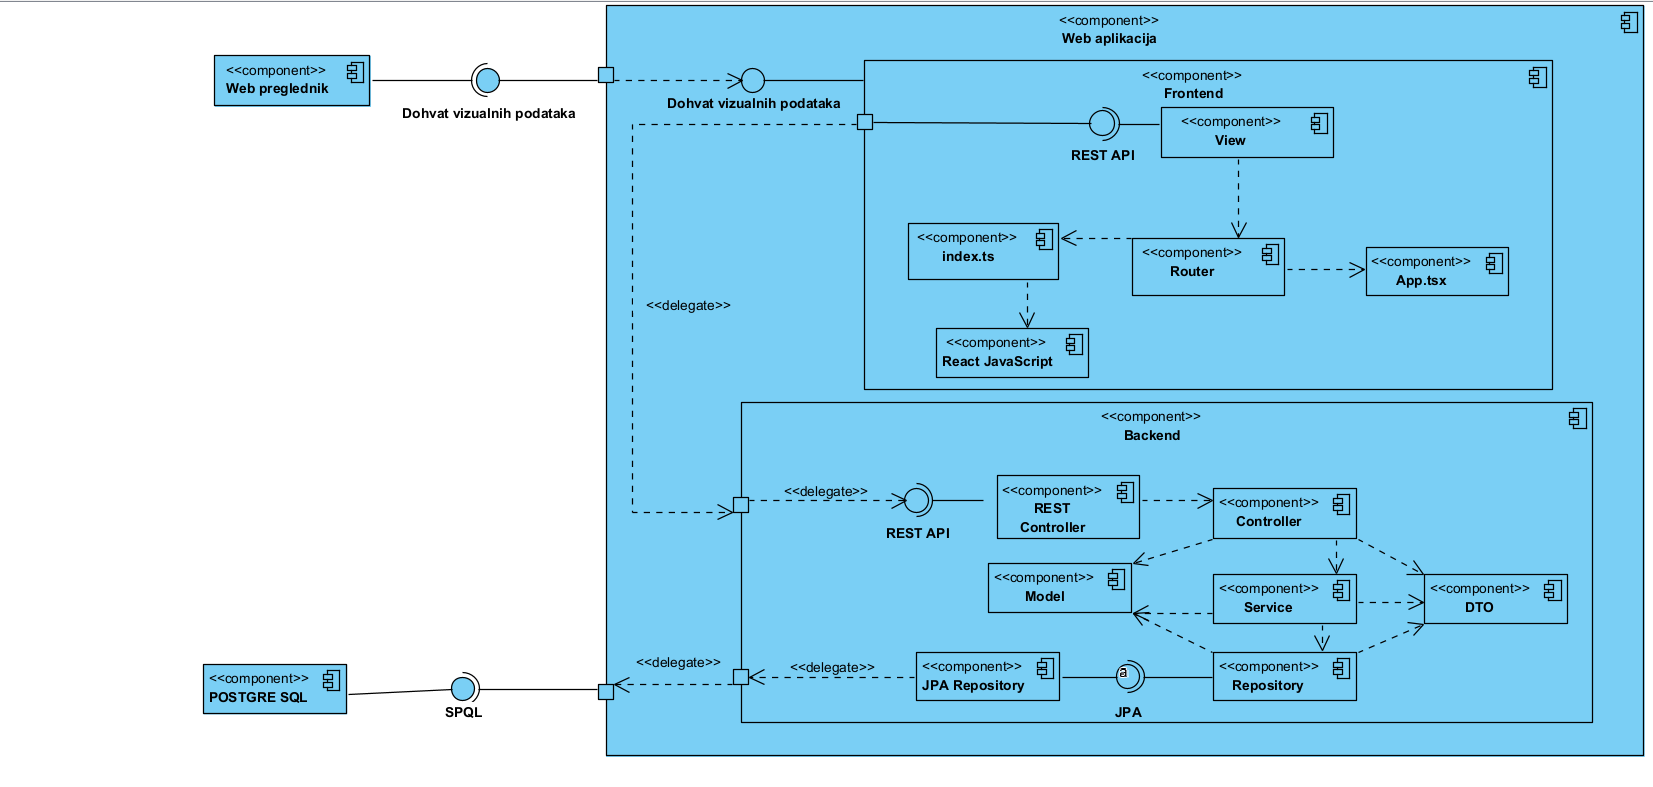
\includegraphics[scale=0.5]{slike/compDiagram.PNG} %veličina slike u odnosu na originalnu datoteku i pozicija slike
			\centering
			\caption{Dijagram komponenti}
			\label{fig:bazapod}
		\end{figure}